\chapter{Testování}
\label{-testovani}

Po vytvoření výpočetních nástrojů bylo provedeno ověření správnosti jejich funkce a posouzení přesnosti použitých metod. Cílem testování bylo prokázat, že chyby zavedené jednotlivými výpočetními postupy jsou ve srovnání s~očekávanými rozdíly analyzovaných veličin dostatečně malé, a nemají tedy zásadní vliv na interpretaci výsledků.

\section{Přesnost určení parametrů časových řad}

Vzhledem k~charakteru použitých metod bylo samostatné testování zaměřeno především na spektrální analýzu, u~níž bylo ověřováno správné určení známých periodických složek v~synteticky generovaných datech. Odhad trendů je založen na standardní metodě nejmenších čtverců, která nebyla samostatně testována. Model se zlomy i~metody detekce diskontinuit byly ověřeny vzájemným porovnáním výsledků jednotlivých metod při analýze reálných časových řad, která je popsána v~kapitole~\ref{sec:casove-rady}.

\subsection{Testování spektrální analýzy}

V~této části je ověřena funkčnost algoritmů \zk{FFT} a~Lomb--Scargleova periodogramu na syntetické časové řadě se známými periodickými složkami. Testovací řada byla vytvořena jako součet tří sinusových funkcí se známými periodami a~amplitudami, které jsou uvedeny v~tabulce~\ref{tab:known_periodicities}, a~náhodného šumu.

\begin{table}[H]
\centering
\caption{Parametry generovaných periodických složek.}
\label{tab:known_periodicities}
\begin{tabular}{lrr}
\toprule
Název & Perioda [dny] & Amplituda [mm] \\
\midrule
půlroční & 182.625 & 5.000 \\
roční & 365.250 & 10.000 \\
200 dní & 200.000 & 7.000 \\
\bottomrule
\end{tabular}
\end{table}


\noindent Výsledná testovací časová řada je znázorněna na
obrázku~\ref{fig:test_data}.

\begin{figure}[H]
  \centering
  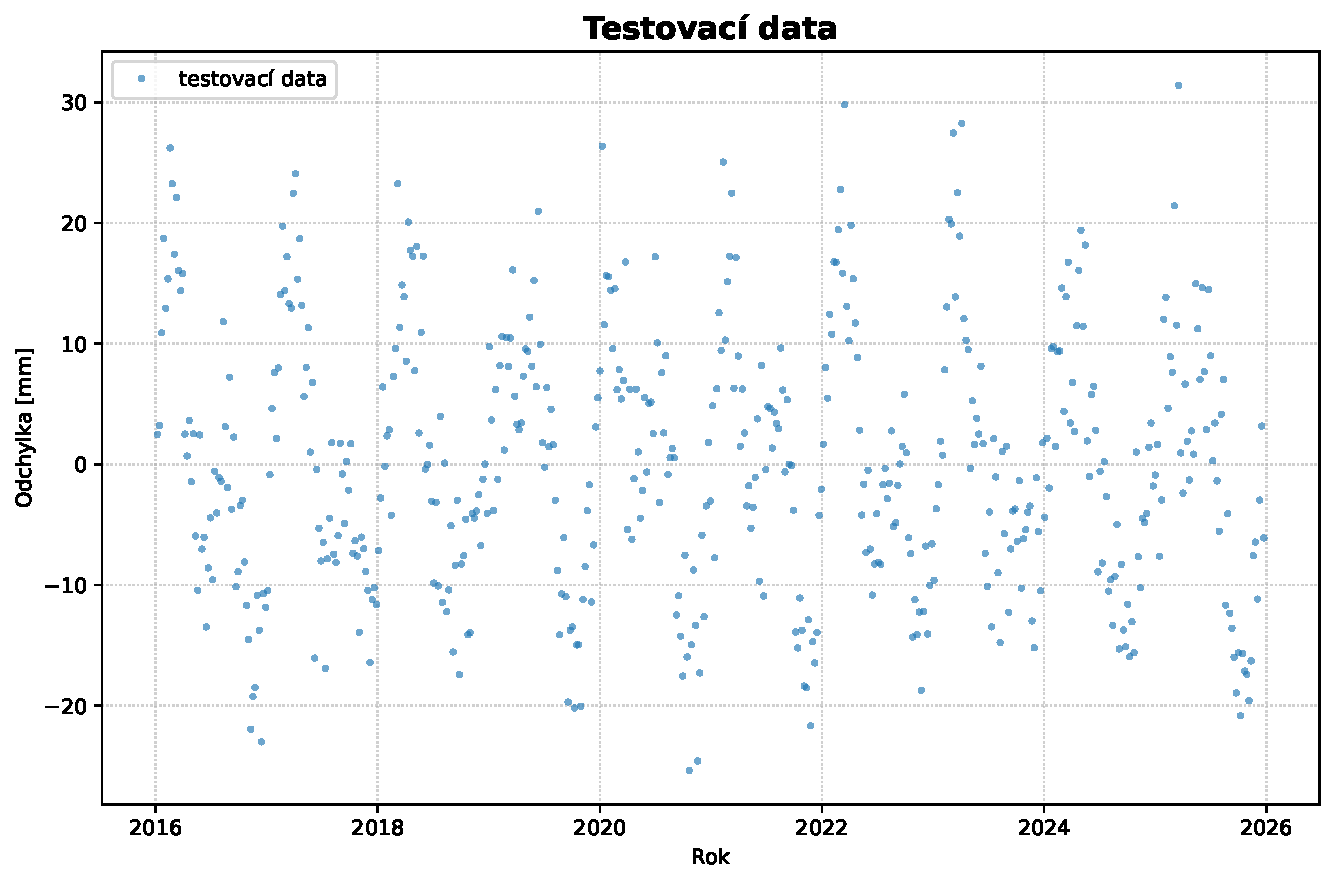
\includegraphics[width=1\linewidth]{images/test/periodicities/test_data.pdf}
  \caption{Syntetická časová řada s~třemi periodickými složkami a šumem}
  \label{fig:test_data}
\end{figure}

\paragraph{FFT periodogram}\leavevmode\\
Pomocí Fourierovy transformace byl vypočten periodogram, ze kterého byly identifikovány dominantní frekvence. Detekované periodicity jsou uvedeny v~tabulce~\ref{tab:fft_significant_peaks}.

\begin{table}[H]
\centering
\small
\caption{Periodické složky detekované metodou FFT.}
\label{tab:fft_significant_peaks}
\begin{tabular}{rrr}
\toprule
Perioda [roky] & Perioda [dny] & Amplituda [mm] \\
\midrule
0.99918 & 364.950 & 10.673 \\
0.55510 & 202.750 & 6.367 \\
0.49959 & 182.475 & 4.679 \\
\bottomrule
\end{tabular}
\end{table}


\noindent Na obrázku~\ref{fig:fft_periodogram} je zobrazen \zk{FFT} periodogram testovacích dat.

\begin{figure}[H]
\centering

\includegraphics[width=1\linewidth]{images/test/periodicities/fft_periodogram.pdf}
\caption{FFT periodogram syntetické časové řady}
\label{fig:fft_periodogram}
\end{figure}


\paragraph{Lomb--Scargleův periodogram}\leavevmode\\
Stejná data byla analyzována pomocí Lomb--Scargleova periodogramu, který je vhodný i pro nepravidelně vzorkované časové řady. Detekované periodicity jsou uvedeny v~tabulce~\ref{tab:lomb_significant_peaks}.

\begin{table}[H]
\centering
\small
\caption{Periodické složky detekované Lomb--Scargleovou metodou.}
\label{tab:lomb_significant_peaks}
\begin{tabular}{rrr}
\toprule
Perioda [roky] & Perioda [dny] & Amplituda [mm] \\
\midrule
1.00156 & 365.819 & 10.693 \\
0.55015 & 200.942 & 6.629 \\
0.49599 & 181.160 & 4.812 \\
1.16689 & 426.208 & 3.439 \\
\bottomrule
\end{tabular}
\end{table}


\noindent Na obrázku~\ref{fig:lomb_periodogram} je znázorněn Lomb--Scargleův periodogram.

\begin{figure}[H]
\centering

\includegraphics[width=1\linewidth]{images/test/periodicities/lomb_scargle_periodogram.pdf}
\caption{Lomb--Scargleův periodogram syntetické časové řady}
\label{fig:lomb_periodogram}
\end{figure}

\paragraph{Zhodnocení výsledků spektrální analýzy}\leavevmode\\
Obě metody úspěšně identifikovaly všechny tři periodické složky přítomné v~testovacích datech. Detekované periody se od skutečných hodnot ve všech případech lišily maximálně v~řádu jednotek dní a~nalezené amplitudy se od skutečných hodnot lišily maximálně v~řádu jednotek milimetrů.

Lomb--Scargleův periodogram má oproti metodě \zk{FFT} výhodu v~tom, že jej lze použít i~pro nepravidelně vzorkované časové řady. V~provedeném testu však detekoval navíc periodicitu o~délce přibližně 426~dní, která v~generovaných datech reálně obsažena nebyla. Metoda \zk{FFT} tuto falešnou periodicitu nedetekovala a~pro pravidelně vzorkovaná data se tak v~provedeném testu jevila jako spolehlivější.

V~dalších analýzách budou proto využívány obě metody vzájemně se doplňujícím způsobem --- \zk{FFT} jako primární nástroj pro pravidelně vzorkované řady a~Lomb--Scargleův periodogram v~případech, kdy jsou v~datech přítomny výpadky nebo nepravidelné vzorkování.

\section{Ověření přesnosti interpolace drah}

Pro porovnání drah družic je nutné převést jednotlivá řešení na společné časové epochy, což lze realizovat například matematickou interpolací. Přesnost interpolace je přitom závislá na zvolené interpolační metodě, charakteru skutečné dráhy družice, hustotě vzorkování a přesnosti vstupních dat. V~ideálním případě nerušeného keplerovského pohybu je dráha družice elipsou a polohu družice by tak bylo možné v~libovolné epoše určit přesně. V~reálných podmínkách je však pohyb družice ovlivněn řadou gravitačních i negravitačních sil, které způsobují odchylky od eliptické dráhy a nelze jej proto dokonale matematicky modelovat.

Pro ověření numerické přesnosti Hermitovy interpolace bylo využito řešení drah družic, které bylo následně uměle zředěno tak, aby vznikly větší časové rozestupy mezi jednotlivými epochami odpovídající různým intervalům vzorkování. V~těchto epochách byly polohy družice určeny interpolací a~porovnány s~původními hustěji vzorkovanými hodnotami, které sloužily jako reference. Pro testování byla využita orbitální řešení \zk{GOP} a~\zk{SSA} pro všechny dostupné družice v~období prvních 30~dní roku 2024, přičemž testování bylo provedeno pro několik různých délek vstupního intervalu. Velikost interpolační chyby byla hodnocena pomocí základních statistických charakteristik vypočtených z~rozdílů poloh (reziduí), konkrétně aritmetického průměru, \zkratka{RMS} a~\zkratka{RMS}0, a~to v~jednotlivých složkách lokálního orbitálního systému \zk{RTN}. Dále byla z~vektoru prostorové vzdálenosti v~každé epoše vyhodnocena celková polohová chyba vyjádřená jako 3D~\zkratka{RMS}. Jako reprezentativní ukázka výsledků je v~následující části uvedeno řešení \zk{GOP} pro družici \zkratka{SARAL}.

\subsubsection{Průběh odchylek interpolace v~rámci jednoho dne}

Na obrázku~\ref{fig:RTN_differences_single_day} jsou znázorněny odchylky polohy v~jednotlivých složkách \zk{RTN} pro první den roku 2024. Graf zachycuje rozdíly mezi původní referenční dráhou se vzorkováním 60~s~a polohami dopočtenými Hermitovou interpolací z~uměle zředěné dráhy se vstupním intervalem 120~s. Odchylky jsou vyjádřeny v~milimetrech.

\begin{figure}[H]
\centering
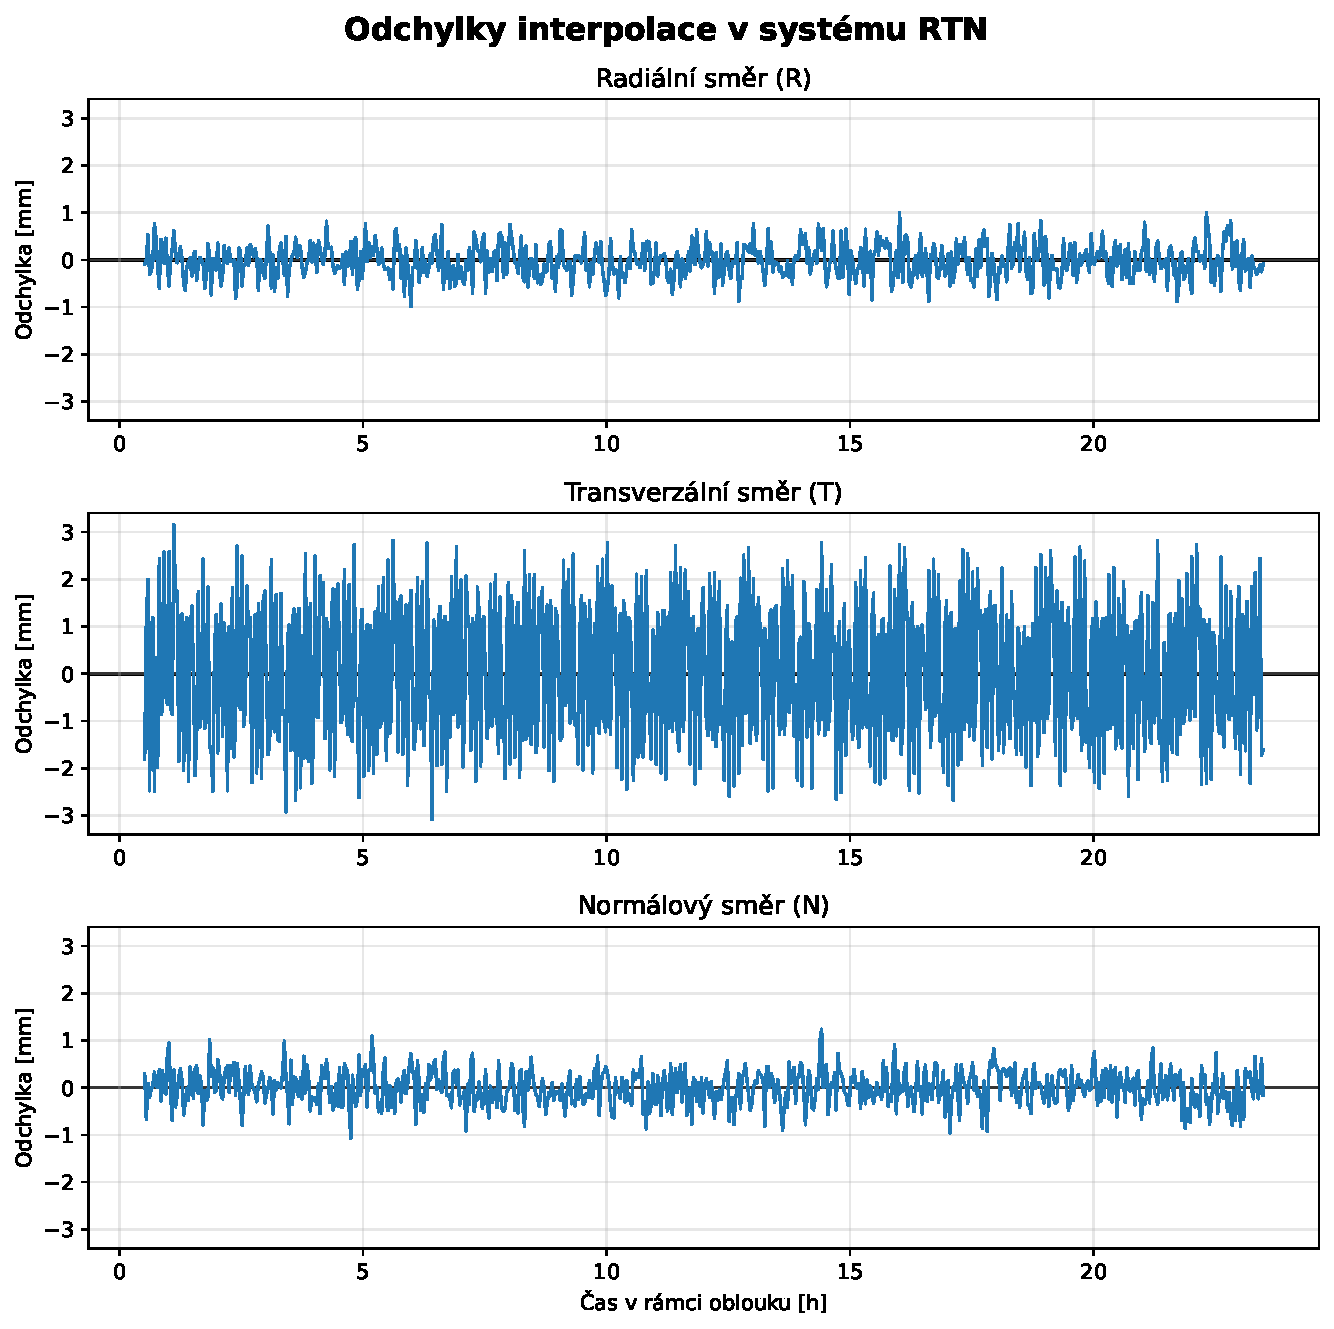
\includegraphics[width=1\linewidth]{images/test/hermite_precision/gop/srl/RTN_differences_single_day.pdf}
\caption{Průběh odchylek interpolace v~systému \zk{RTN} pro 1. 1. 2024}
\label{fig:RTN_differences_single_day}
\end{figure}

Z~obrázku je patrné, že rozdíly interpolované polohy mají hladký průběh bez výrazných skoků. Největší odchylky se vyskytují v~transverzální složce T, která odpovídá směru letu družice a je na interpolační chybu nejcitlivější. Maximální hodnoty odchylek v~radiální a normálové složce se pohybují kolem 1~mm, zatímco v~transverzální složce dosahují až přibližně 3~mm.

Pro podrobnější analýzu charakteru odchylek jsou na obrázku~\ref{fig:RTN_histogram_single_day} uvedeny histogramy jednotlivých složek systému \zk{RTN}. Odchylky jsou vykresleny se zachováním znaménka, což umožňuje posoudit jejich symetrii vzhledem k~nulové hodnotě.

\begin{figure}[H]
\centering
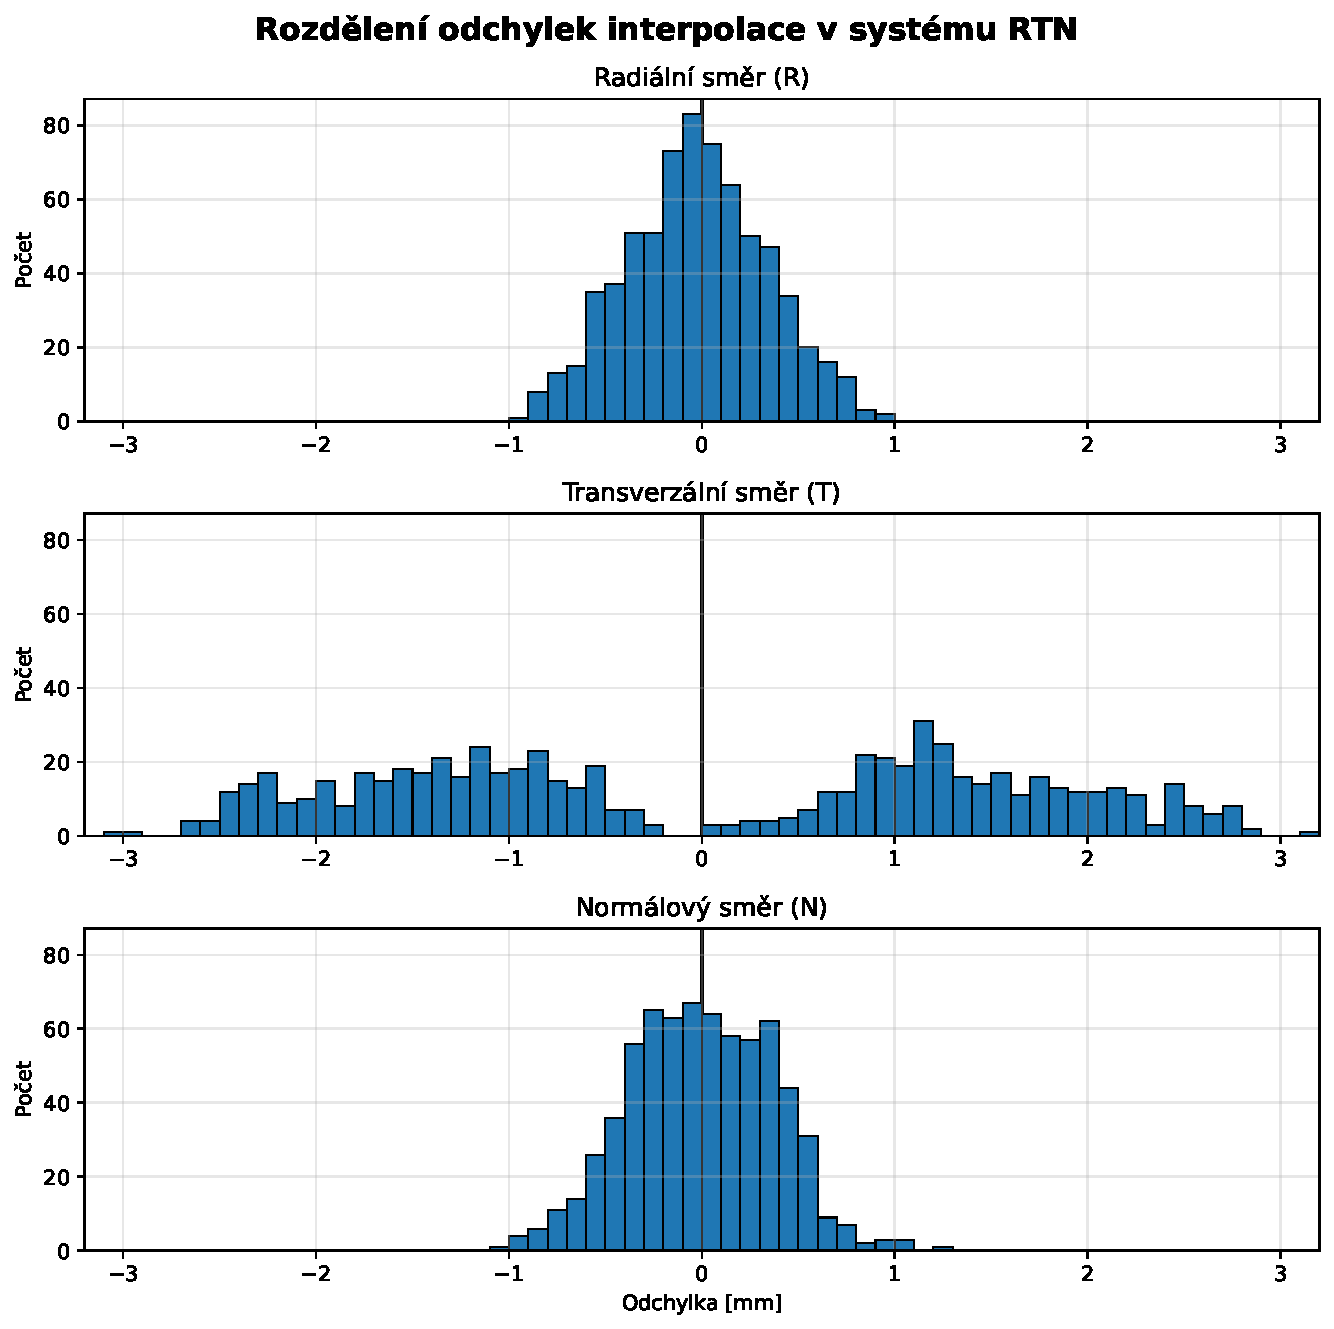
\includegraphics[width=1\linewidth]{images/test/hermite_precision/gop/srl/RTN_histogram_single_day.pdf}
\caption{Histogramy odchylek interpolace v~systému \zk{RTN} pro 1. 1. 2024}
\label{fig:RTN_histogram_single_day}
\end{figure}

Z~histogramů je patrné, že se charakter rozdělení odchylek v~jednotlivých složkách liší. V~radiální a normálové složce jsou odchylky soustředěny v~blízkosti nulové hodnoty a jejich rozsah je výrazně menší než v~transverzálním směru. Naproti tomu v~transverzální složce je rozdělení širší a vykazuje nepravidelný charakter s~častějším výskytem hodnot mimo okolí nulové hodnoty. Vyšší odchylky v~této složce souvisí s~tím, že transverzální směr odpovídá směru letu, který je nejcitlivější na nepřesnosti v~aproximaci trajektorie a vstupních rychlostech Hermitovy interpolace. Odlišný tvar rozdělení v~této složce může naznačovat přítomnost systematické chyby.

Na obrázku~\ref{fig:interp_periodogram} jsou zobrazeny periodogramy odchylek v~jednotlivých složkách systému \zk{RTN}, které slouží k~identifikaci periodických složek v~chybách interpolace.

\begin{figure}[H]
\centering
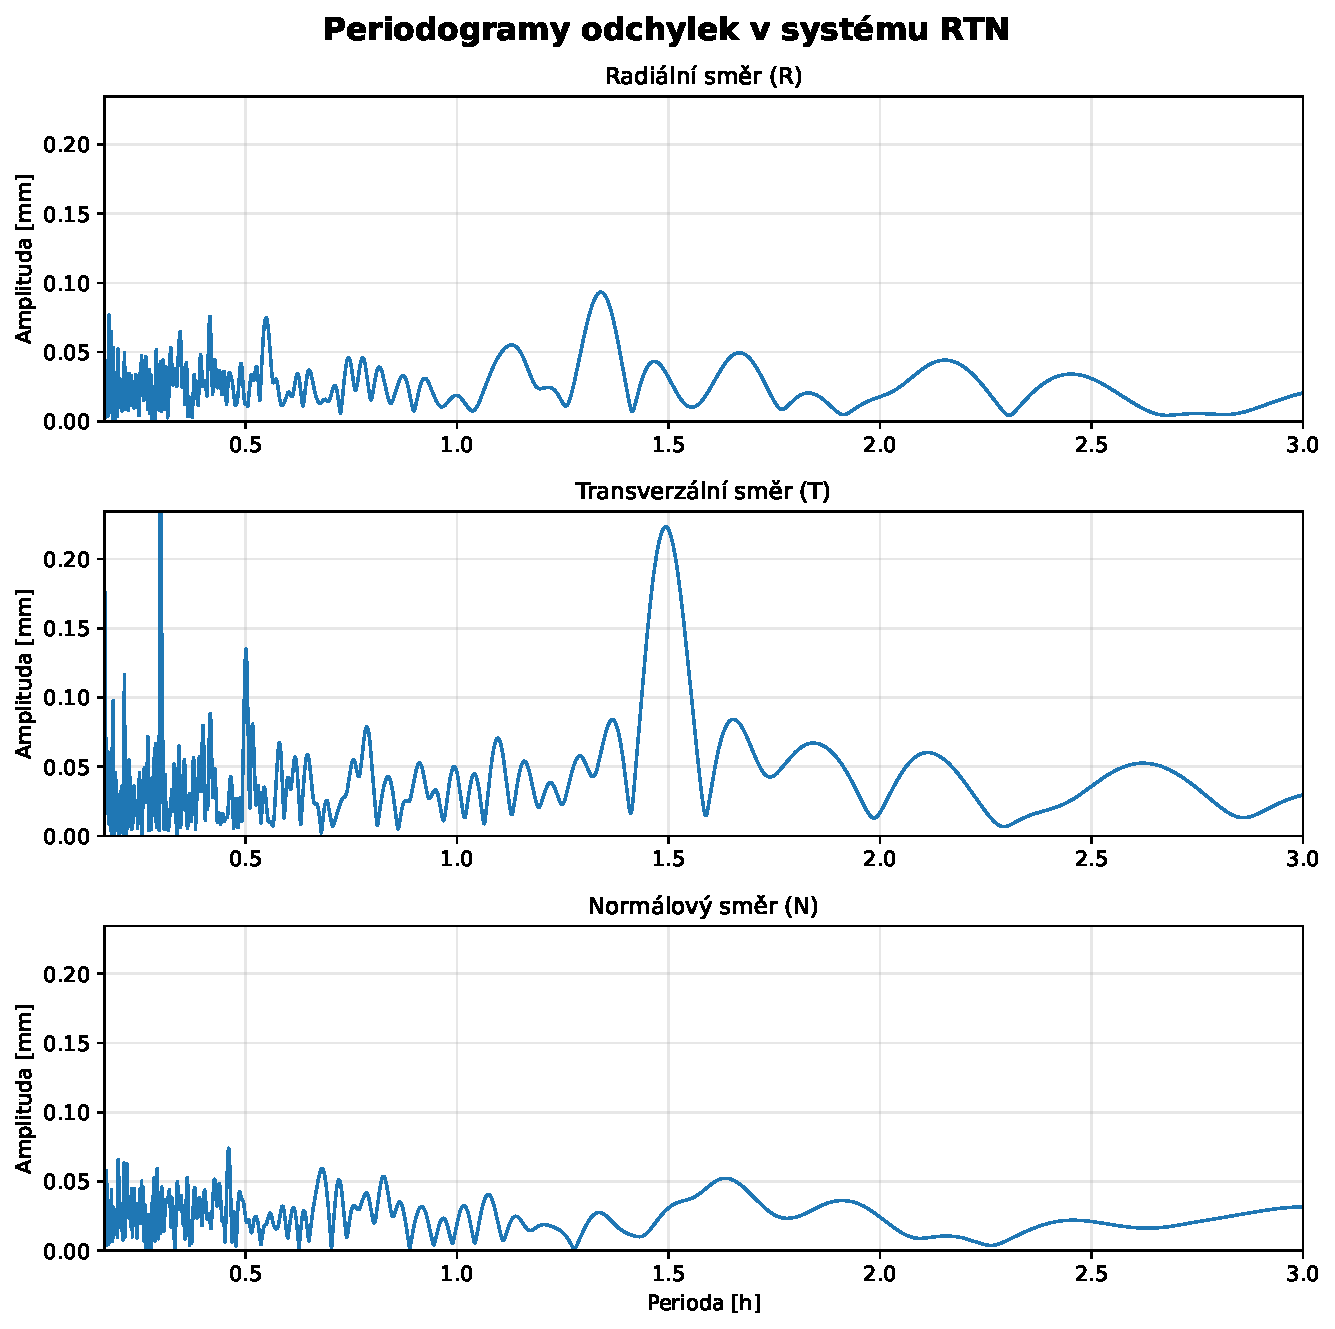
\includegraphics[width=1\linewidth]{images/test/hermite_precision/gop/srl/RTN_lomb_scargle_periodograms_single_day.pdf}
\caption{Periodogramy odchylek interpolace v~systému \zk{RTN} pro 1.~1.~2024}
\label{fig:interp_periodogram}
\end{figure}

Z~periodogramů je patrné, že v~radiální a normálové složce se nevyskytují výrazné dominantní periodicity. Naproti tomu v~transverzální složce je patrná periodická složka s~periodou přibližně 1{,}5~hodiny a amplitudou v~řádu desetin milimetru. Tato perioda přibližně odpovídá oběžné době družice \zkratka{SARAL}, která činí přibližně 100{,}5~minuty. V~grafu je současně patrná také výraznější složka s~periodou kolem 20~minut. Tyto periodicity naznačují, že část interpolační chyby v~transverzálním směru nemá čistě náhodný charakter.

\subsubsection{Stabilita interpolační chyby v~čase}

Pro posouzení stability chyby interpolace ve složkách \zk{RTN} v~delším časovém období byly analyzovány denní hodnoty \zkratka{RMS} pro vstupní interval 120~s. Na obrázku~\ref{fig:Daily_RTN_RMS_over_time} je znázorněn jejich průběh od 1.~1.~2024 do 30.~1.~2024.

\begin{figure}[H]
\centering
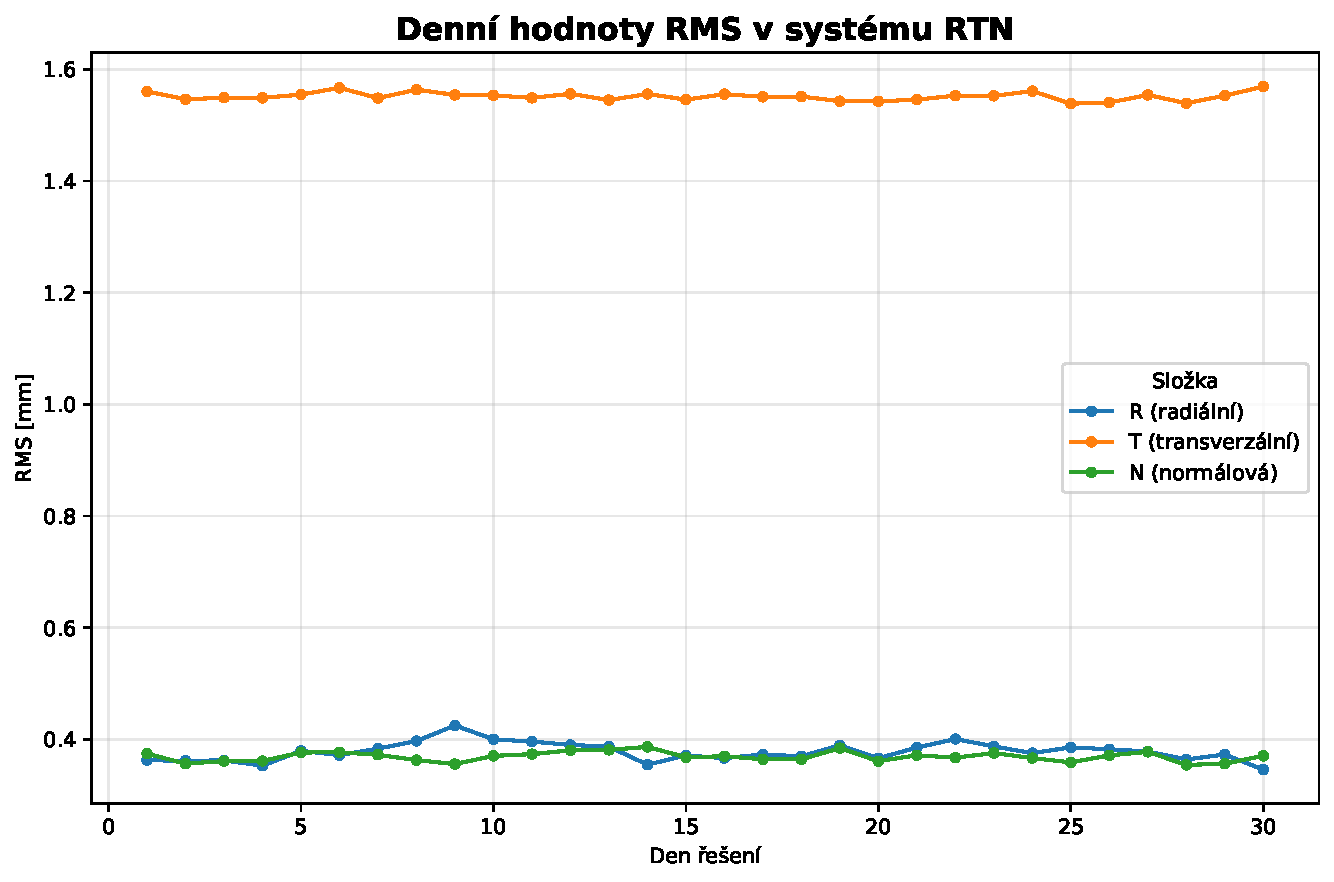
\includegraphics[width=1\linewidth]{images/test/hermite_precision/gop/srl/Daily_RTN_RMS_over_time.pdf}
\caption{Denní hodnoty \zk{RMS} v~systému \zk{RTN} pro vstupní interval 120~s}
\label{fig:Daily_RTN_RMS_over_time}
\end{figure}

Z~grafu je patrné, že hodnoty \zkratka{RMS} v~radiální a normálové složce se stabilně pohybují kolem 0{,}4~mm, zatímco v~nejcitlivější transverzální složce dosahují přibližně 1{,}5~mm. Rezidua jsou v~čase stabilní, bez patrných trendů či skoků. To naznačuje, že použitá Hermitova interpolace 11.~řádu poskytuje v~celém analyzovaném období vnitřně konzistentní výsledky.

\subsubsection{Závislost interpolační chyby na délce vstupního intervalu}

Pro posouzení vlivu vzorkovacího intervalu na přesnost interpolace byla analyzována závislost prostorové chyby na časovém kroku mezi vstupními epochami. Na obrázku~\ref{fig:Daily_3D_RMS_over_time} jsou znázorněny denní hodnoty 3D \zkratka{RMS} pro vybrané intervaly v~průběhu prvních 30~dní roku 2024.

\begin{figure}[H]
\centering
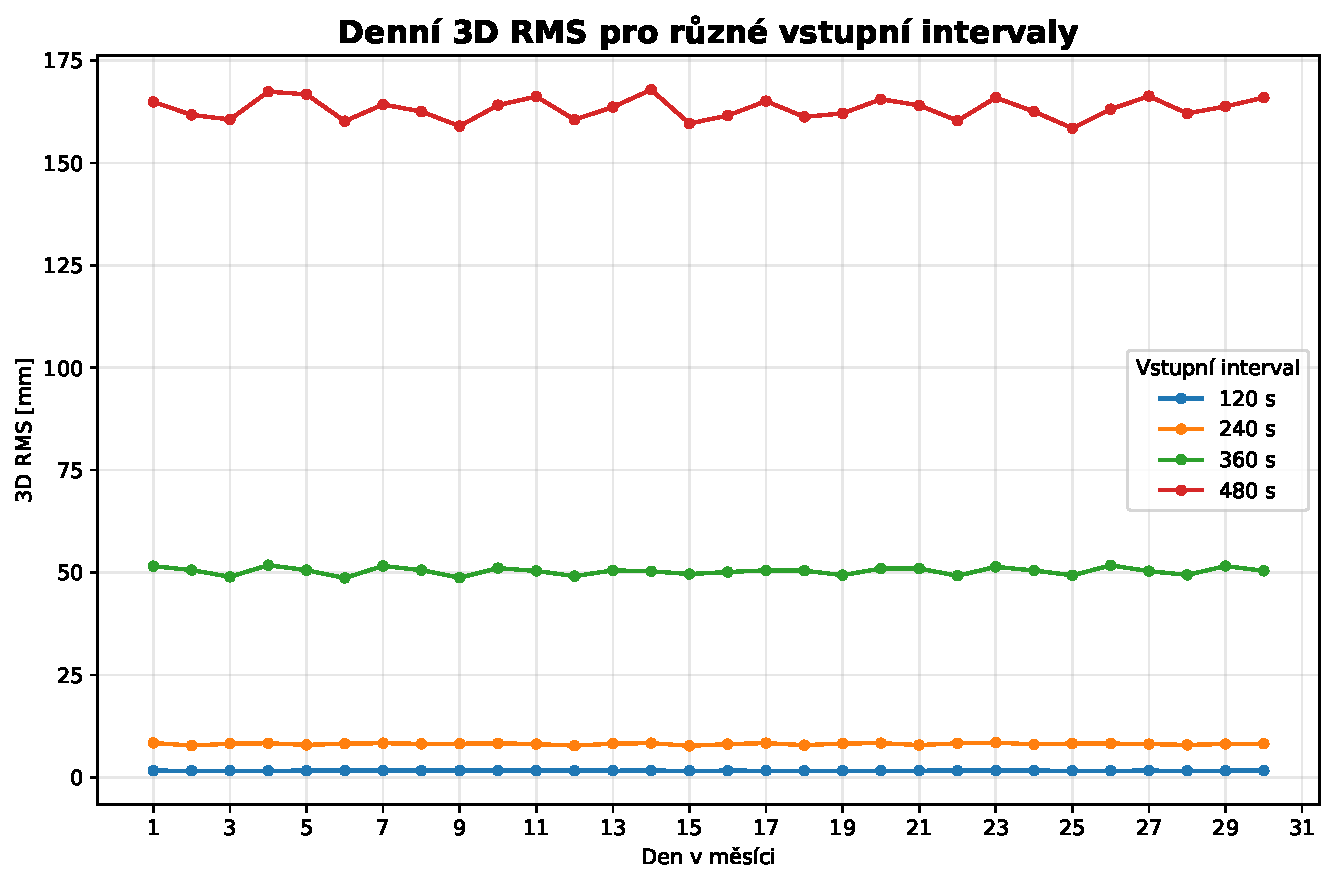
\includegraphics[width=1\linewidth]{images/test/hermite_precision/gop/srl/Daily_3D_RMS_over_time.pdf}
\caption{Denní 3D \zk{RMS} pro různé vstupní intervaly}
\label{fig:Daily_3D_RMS_over_time}
\end{figure}

Z~grafu je patrné, že velikost chyby interpolace výrazně závisí na délce vstupního intervalu. Pro 120~s~dosahuje 3D \zkratka{RMS} nižších jednotek milimetrů, pro 240~s~vyšších jednotek milimetrů a pro 360~s~až 480~s~již desítek až stovek milimetrů. Hodnoty jsou v~čase stabilní, což potvrzuje, že hlavním faktorem přesnosti je délka vstupního intervalu.

Pro kvantitativní shrnutí výsledků jsou v~tabulce~\ref{tab:interp_accuracy} uvedeny souhrnné hodnoty \zk{RMS} interpolační chyby pro jednotlivé vstupní intervaly.

\begin{table}[H]
\centering
\small
\caption{Souhrnné statistiky interpolační chyby pro různé vstupní intervaly}
\label{tab:interp_accuracy}
\begin{tabular}{rrrrr}
\toprule
Interval [s] & R [mm] & T [mm] & N [mm] & 3D RMS [mm] \\
\midrule
120 & 0.378 & 1.552 & 0.369 & 1.639 \\
240 & 5.690 & 5.588 & 1.725 & 8.159 \\
360 & 35.957 & 33.530 & 10.910 & 50.360 \\
480 & 115.936 & 109.275 & 35.632 & 163.254 \\
\bottomrule
\end{tabular}
\end{table}


Z~tabulky je patrné, že s~rostoucím vstupním intervalem dochází k~výraznému nárůstu chyby ve všech složkách systému \zk{RTN}. Pro uměle zředěný interval 120~s~se chyba pohybuje v~řádu milimetrů. V~radiální a normálové složce nepřesahuje 0{,}4~mm a v~transverzální složce dosahuje přibližně 1{,}6~mm. U~delších intervalů chyba narůstá nelineárně a pro krok 480~s~dosahuje celková hodnota 3D \zkratka{RMS} přibližně 163~mm. Tabulka tak potvrzuje, že přesnost interpolace je silně závislá na hustotě vzorkování vstupních epoch.

\subsubsection{Odhad přesnosti pro interval 60~s}

Pro doplnění hodnocení přesnosti byla aproximována závislost celkové chyby 3D \zk{RMS} na délce vstupního intervalu. Výsledná závislost je znázorněna na obrázku~\ref{fig:RMS_3D_vs_interval_estimate}.

\begin{figure}[H]
\centering
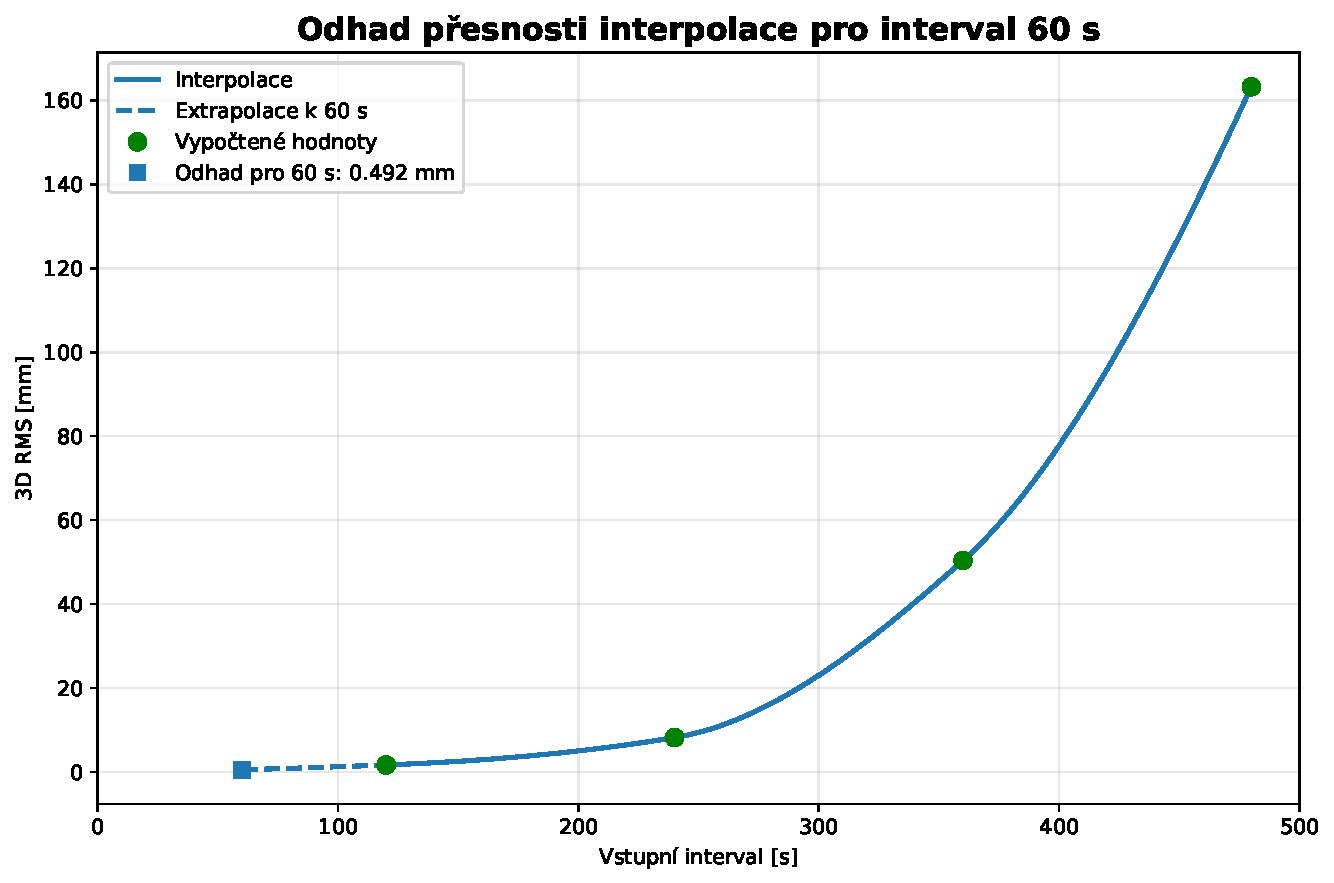
\includegraphics[width=1\linewidth]{images/test/hermite_precision/gop/srl/RMS_3D_vs_interval_estimate_60s.pdf}
\caption{Závislost 3D \zk{RMS} na délce vstupního intervalu}
\label{fig:RMS_3D_vs_interval_estimate}
\end{figure}

Plná část křivky byla interpolována mezi hodnotami vypočtenými pro vstupní intervaly 120--480~s~a znázorňuje nelineární charakter růstu chyby. Přerušovaná část křivky představuje extrapolaci směrem k~intervalu 60~s. Výsledná odhadnutá hodnota 3D \zkratka{RMS} pro interval 60~s~je přibližně 0{,}49~mm. Tato hodnota odpovídá celkovému trendu pozorovanému v~datech a naznačuje, že při vstupním intervalu 60~s~lze očekávat submilimetrovou přesnost interpolace. Uvedený výsledek však nebyl přímo ověřen nezávislou referencí s~hustším vzorkováním, a představuje proto pouze orientační odhad.

\subsubsection{Shrnutí}

Hermitova interpolace poskytuje stabilní výsledky, jejichž přesnost narůstá s~klesajícím intervalem vzorkování. Největší odchylky se vyskytují v~transverzální složce, kde při vzorkování 120~s~nepřesahují jednotky milimetrů (3D \zkratka{RMS} 1{,}6~mm). S~delším intervalem roste chyba nelineárně až na stovky milimetrů. Extrapolace pro krok 60~s~indikuje submilimetrovou přesnost, která by již výrazně neovlivňovala výsledky porovnání drah družic.

\section{Ověření přesnosti parametrizace drah}

Pro ověření přesnosti dynamické parametrizace drah byly bodové dráhy ve formátu \texttt{SP3} parametrizovány v~softwaru Bernese pomocí modulu \texttt{ORBGEN}. Výstupem jsou soubory \texttt{.OUT}, které obsahují statistiky přesnosti parametrizace a~rezidua dynamicky parametrizované dráhy vůči referenčním bodům ze souboru \texttt{SP3} v~lokálním orbitálním systému \zk{RTN}.

Testování bylo provedeno na řešení \zk{SSA} pro družici \zkratka{SARAL} za prvních 30~dní roku 2024. Výpočet byl realizován ve dvou iteracích. Pro testování bylo zvoleno řešení \zk{SSA}, protože řešení \zk{GOP} bylo již určeno pomocí dynamické parametrizace v~softwaru Bernese a~opakovaná parametrizace by tak mohla vést k~nadhodnocení dosažené přesnosti. Přesnost parametrizace byla hodnocena pomocí \zkratka{RMS} reziduí v~jednotlivých složkách systému \zk{RTN} a~celkové prostorové chyby vyjádřené jako 3D~\zkratka{RMS}.

Cílem testování bylo ověřit, zda dynamická parametrizace nezavádí do výsledných drah významné systematické chyby a~zda dosažená přesnost postačuje pro následné porovnání jednotlivých orbitálních řešení.

\subsubsection{Průběh odchylek v~rámci jednoho dne}

Na obrázku~\ref{fig:za_rtn_residuals} je znázorněn průběh epochových reziduí ve složkách
\zk{RTN} pro první den roku 2024.

\begin{figure}[H]
\centering
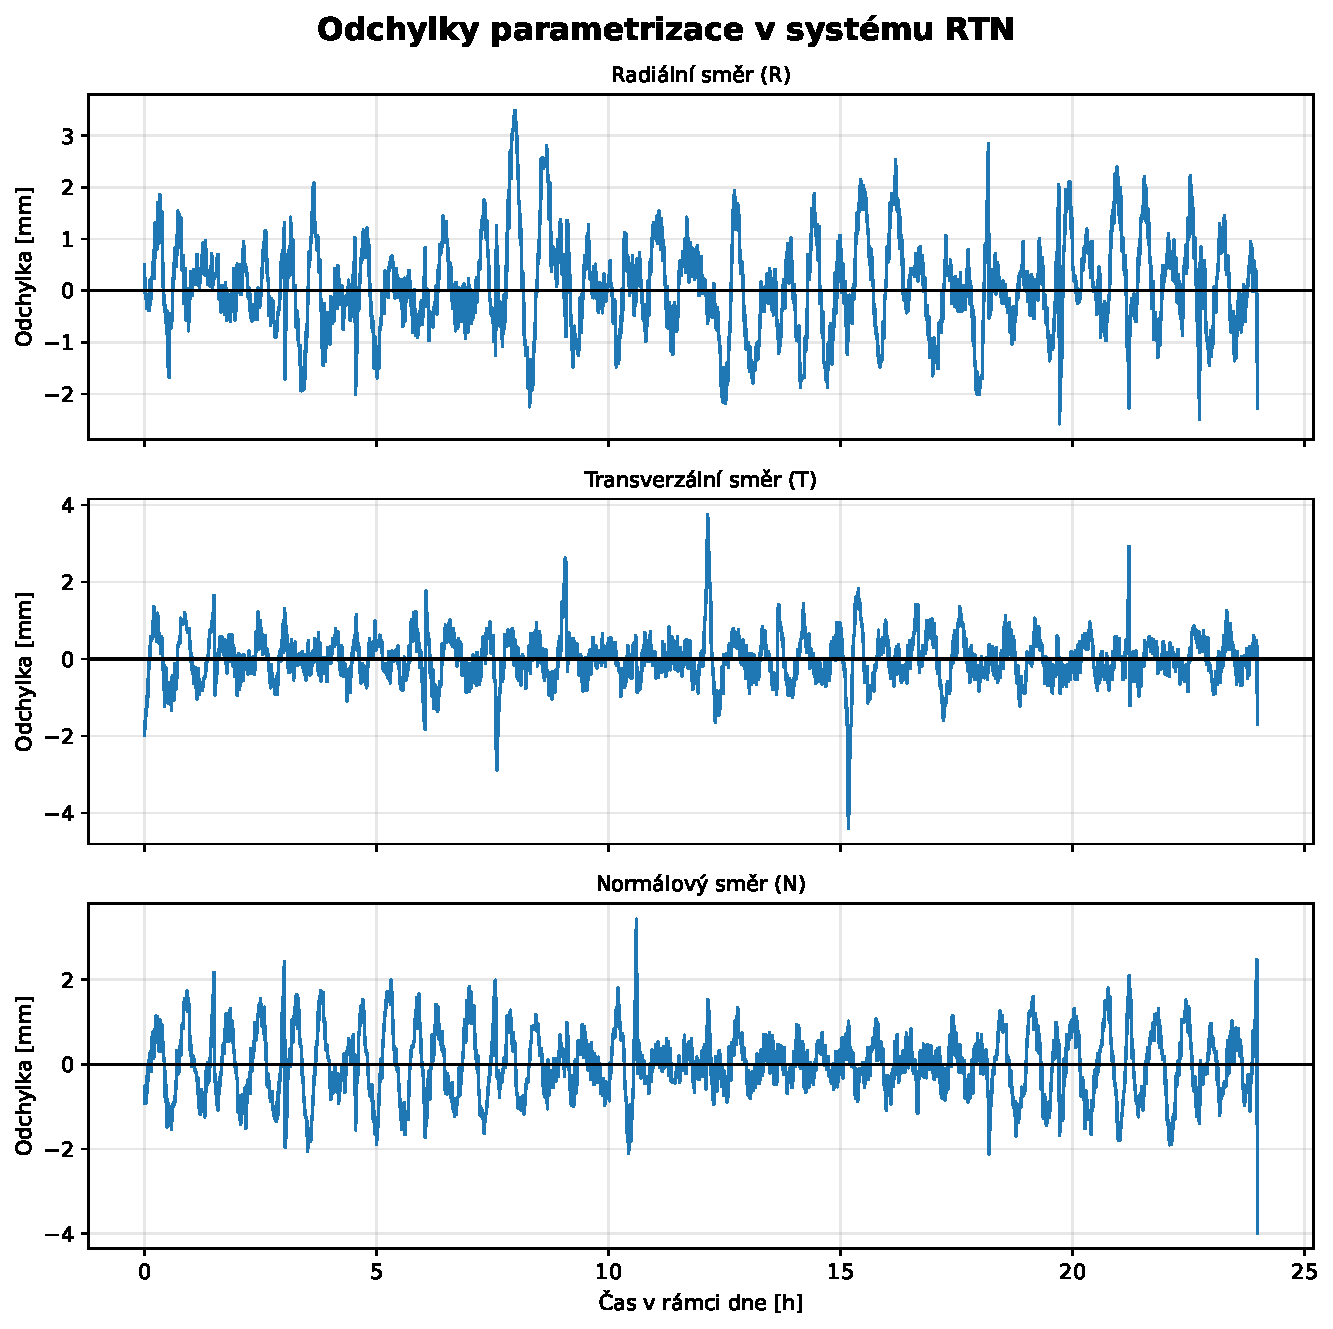
\includegraphics[width=1\linewidth]{images/test/dynamic_precision/sa_za_rtn_residuals_doy001_iter2.pdf}
\caption{Průběh odchylek parametrizace v~systému \zk{RTN} pro 1.~1.~2024}
\label{fig:za_rtn_residuals}
\end{figure}

Z~grafu je patrné, že odchylky mají plynulý průběh bez výrazných skoků, přičemž jejich
charakter se mění v~závislosti na konkrétním dynamickém oblouku. Odchylky v~radiální
složce dosahují hodnot až přibližně 3,5~mm, v~transverzální složce pak až 4,4~mm
a v~normálové složce do~4~mm.

Pro posouzení statistického rozložení odchylek jsou na obrázku~\ref{fig:za_rtn_histograms}
znázorněny histogramy reziduí v~jednotlivých složkách \zk{RTN}.

\begin{figure}[H]
\centering
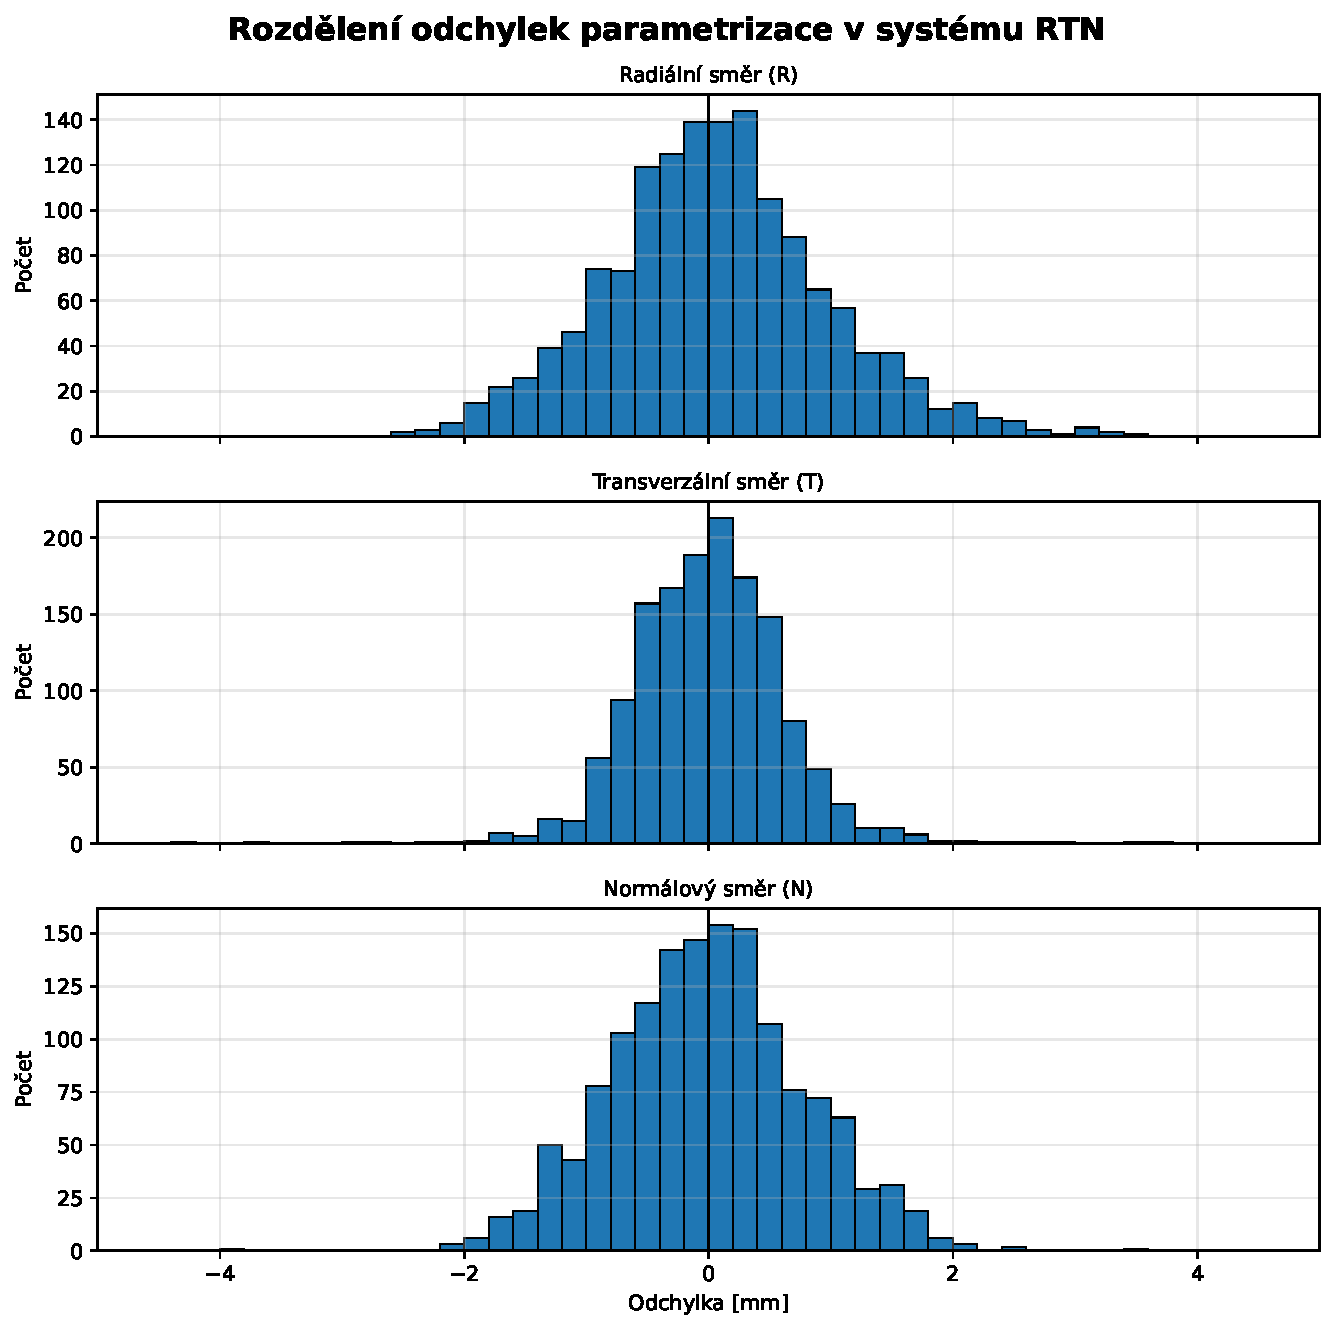
\includegraphics[width=1\linewidth]{images/test/dynamic_precision/sa_za_rtn_histograms_doy001_iter2.pdf}
\caption{Histogramy odchylek parametrizace v~systému \zk{RTN} pro 1.~1.~2024}
\label{fig:za_rtn_histograms}
\end{figure}

Z~histogramů je patrné, že odchylky jsou ve všech třech složkách soustředěny v~blízkosti
nulové hodnoty a vykazují přibližně symetrické rozdělení. Tento charakter naznačuje
absenci výrazných systematických odchylek.

\subsubsection{Spektrální analýza odchylek}

Pro identifikaci případných periodických složek v~odchylkách parametrizace byl vypočten
Lombův--Scargleův periodogram epochových reziduí. Na obrázku~\ref{fig:za_rtn_periodograms}
jsou znázorněny periodogramy pro složky \zk{RTN}.

\begin{figure}[H]
\centering
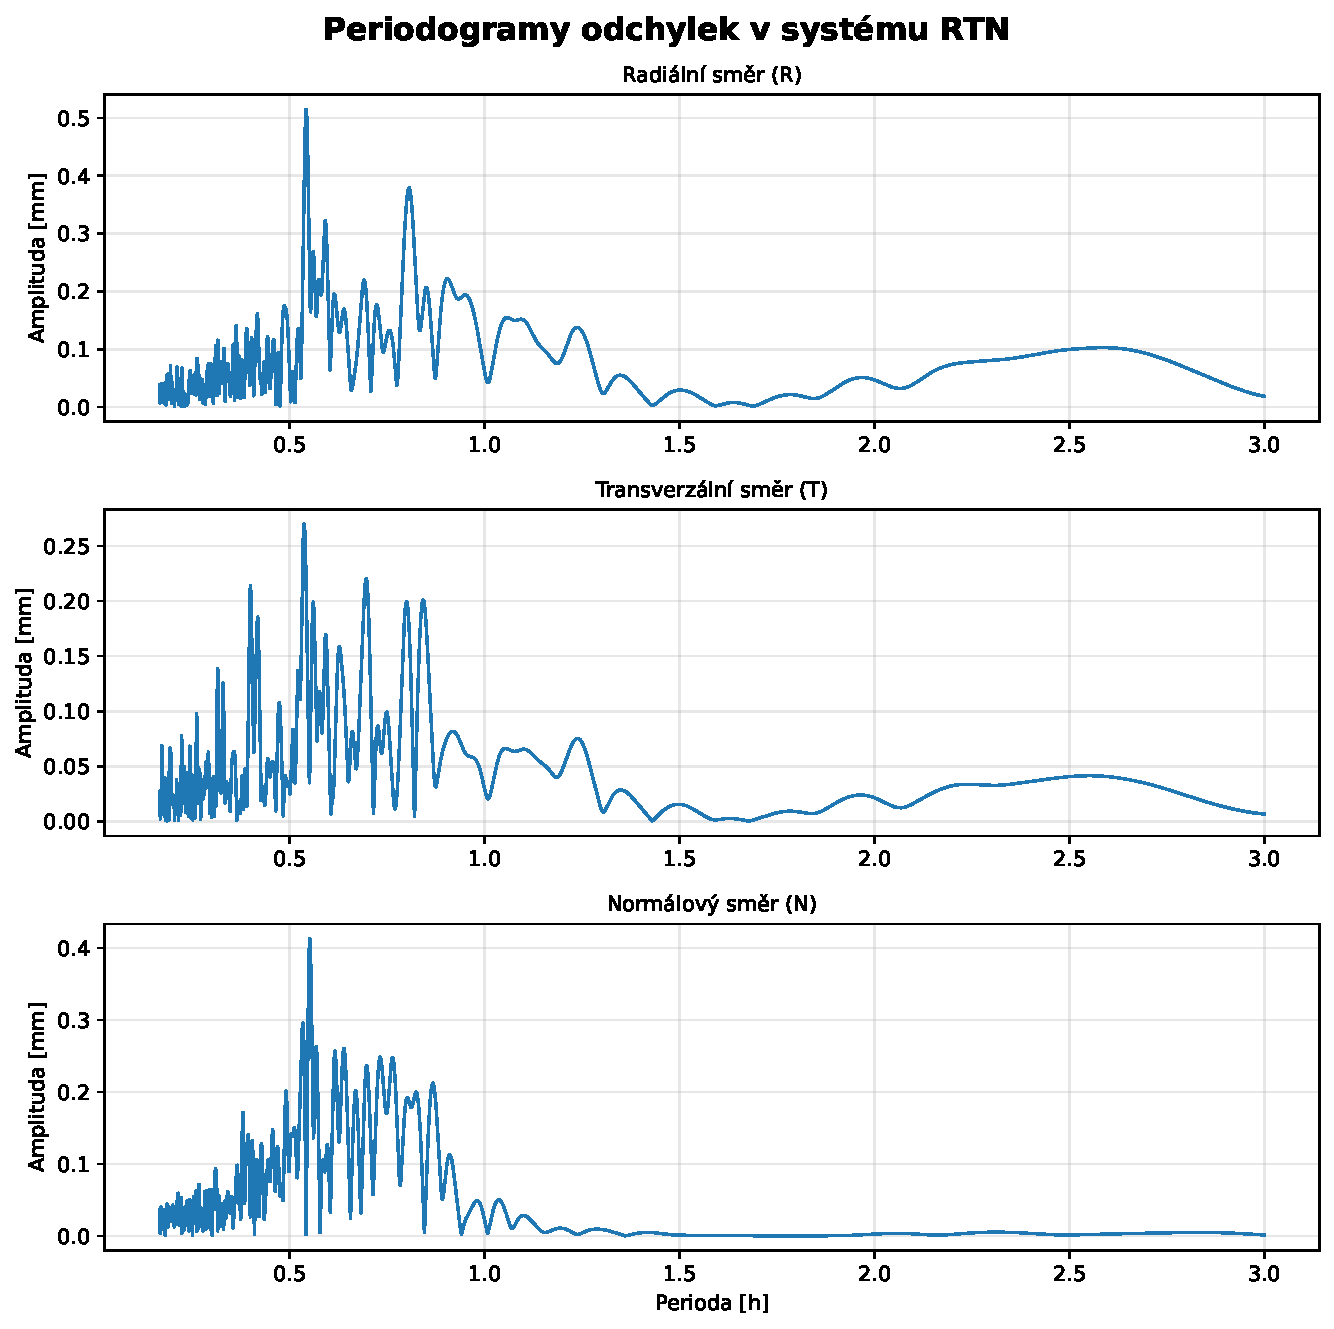
\includegraphics[width=1\linewidth]{images/test/dynamic_precision/sa_za_rtn_periodograms_doy001_iter2.pdf}
\caption{Periodogramy odchylek parametrizace v~systému \zk{RTN} pro 1.~1.~2024}
\label{fig:za_rtn_periodograms}
\end{figure}

Periodogramy naznačují přítomnost několika slabších periodických složek s~periodami přibližně kolem 0{,}5~h a amplitudami řádově v~desetinách milimetru. Tyto složky pravděpodobně nesouvisí přímo s~oběžnou dobou družice \zkratka{SARAL}, která je výrazně delší, ani s~délkou použitého parametrizačního oblouku. Jejich zjevnou příčinu se nepodařilo určit. Vzhledem k~nízkým amplitudám je lze považovat spíše za šum nebo drobný numerický projev parametrizace než za významný zdroj chyb.

\subsubsection{Stabilita přesnosti v~čase}

Pro posouzení časové stability přesnosti jsou na obrázku~\ref{fig:za_daily_rms} znázorněny denní hodnoty \zkratka{RMS} v~průběhu prvních 30~dní roku 2024.

\begin{figure}[H]
\centering
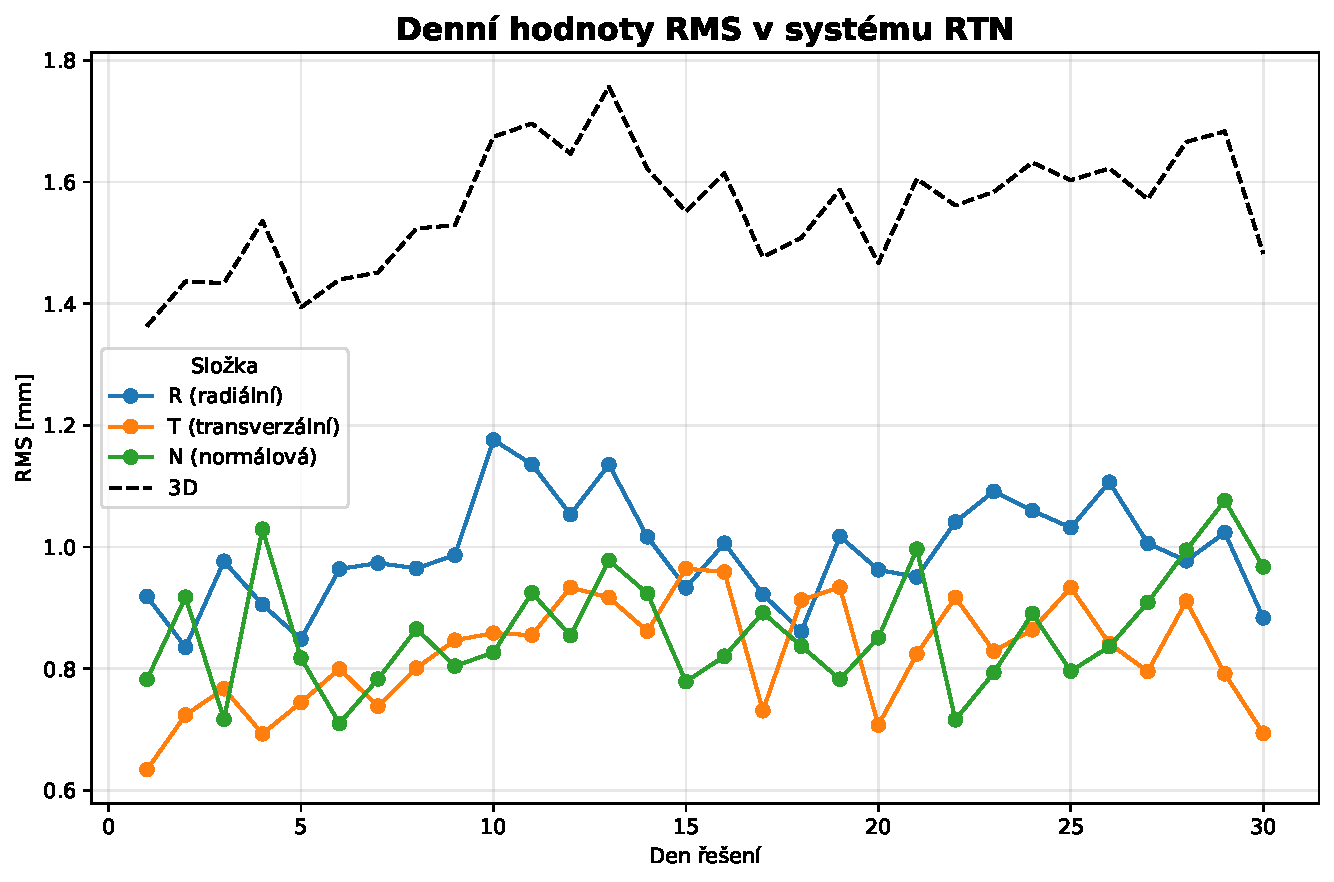
\includegraphics[width=1\linewidth]{images/test/dynamic_precision/sa_za_daily_rms_doy001_030_iter2.pdf}
\caption{Denní hodnoty \zk{RMS} parametrizace v~systému \zk{RTN}}
\label{fig:za_daily_rms}
\end{figure}

Denní hodnoty \zk{RMS} nevykazují výrazné trendy ani skoky, což naznačuje časově stabilní přesnost parametrizace. Souhrnné statistiky vypočtené z~jednotlivých epoch za celé analyzované období (prvních 30~dní roku 2024) jsou uvedeny v~tabulce~\ref{tab:sa_za_rms_summary}.

\begin{table}[H]
\centering
\small
\caption{Souhrnné statistiky parametrizace pro prvních 30~dní roku 2024}
\label{tab:sa_za_rms_summary}
\begin{tabular}{lrrr}
\toprule
Složka & Průměr [mm] & RMS [mm] & Max. abs. reziduum [mm] \\
\midrule
R & 0.104 & 0.996 & 5.460 \\
T & -0.000 & 0.831 & 9.490 \\
N & 0.007 & 0.867 & 23.130 \\
3D & 1.372 & 1.560 & 23.641 \\
\bottomrule
\end{tabular}
\end{table}


\subsubsection{Shrnutí}

Dynamická parametrizace dráhy v~softwaru Bernese vykazuje v~celém analyzovaném období stabilní přesnost. Hodnoty \zk{RMS} epochových reziduí se ve všech složkách systému \zk{RTN} pohybují v~řádu nižších jednotek milimetrů. Spektrální analýza současně neodhalila výrazné periodické složky, což naznačuje absenci významných systematických periodických chyb parametrizace.